\documentclass[10pt]{article}
\usepackage{stat}
\usepackage{graphicx}
\usepackage{setspace}
\usepackage[margin=1.25in]{geometry}
\usepackage{natbib}
\usepackage{todonotes}
\usepackage{imakeidx}
\usepackage{wrapfig}
\bibliographystyle{plainnat}

\title{On \textit{Mechanistic Stability}, Generalization, and Robustness}
\date{\today}

\setlength\parindent{0pt}%
\setlength{\parskip}{3pt}%

\begin{document}

\ifthenelse{\isundefined{\showlinenum}}{
}{
\linenumbers
}
\maketitle

\begin{abstract}
Herein, we introduce a notion which we call \textit{mechanistic stability} which
characterizes the sensitivity of a models' prediction criteria with respect to
perturbations of the task specification.
\end{abstract}

{\fontfamily{lmss}
\begin{spacing}{1}
\tableofcontents
\end{spacing}
}
\clearpage
\setcounter{page}{1}

\allowdisplaybreaks

% !TEX root = ../main.tex 

\section{Defining Mechanistic Staiblity}
At the highest level, \textit{mechanistic stability} is the stability
of a model's decision criteria with respect to changes in the input.
In many cases, we expect a strong, generalizable learner to also be
one that is mechanistically stable. For example, given two-operand
addition problems, we would expect a strong learner to add four-digit
numbers in the same way it adds eight-digit numbers. On the other
hand, a mechanistically stable learner may be necessary for fairness.
Consider a model that evaluates job applicants. A legal and ethical model
must not change its evaluation criteria based on an applicant's gender. 
In this paper, we formalize using tools from category theory, this notion
of mechanistic stability. Then, we show that mechanistic stability is a
sufficient condition for both generalization and robustness. Finally, we
provide a host of empirical results to showcase when mechanistic stability
can be induced or inhibited. Throughout the paper, we use the task of 
two-operand addition as a running
example.

This remainder of this section is organized as follows:
\begin{enumerate}
\item First, in Section~\ref{s:partitioning-subtasks}, we formalize 
what we mean by ``changes in the input'' through
the concept of a \textit{permissible partition} over a data distribution.
\item Then, in Section~\ref{s:causal-equiv}, we define ``stability a model's decision criteria'' through
a category-theoretic equivalence between a model's mechanism on a specific
\textit{permisssible partition}. 
\item FInally, in Section~\ref{s:mech-stab}, by combining these components 
together, we arrive at our
notion of \textit{mechanistic stability}.
\end{enumerate}

Our contribution focuses on the supervised learning regime. Under this setup,
any model's input is chosen from a set $\cX$ and its outputs lie in a set
$\cY$. Let $(\cX, \cF_\cX, \P_\cX)$ and $(\cY, \cF_\cY, \P_\cY)$ be
probability spaces over $\cX, \cY$, respectively. 
Denote by $(\cX \times \cY,
\cF_\cX \otimes \cF_\cY, \P_\cX \times \P_\cY)$ the product probability
space over all input-output pairs. We call any probability measure 
$\P_{\cX\times\cY}$ that is absolutely continuous\footnote{For any
$E \in \cF_\cX\otimes \cF_\cY$, if $(\cP_\cX \times \cP_\cY)(E) = 0$,
then $\P_{\cX\times\cY}(E) = 0$.} to 
$\P_\cX \times \cP_\cY$ a \textit{data distribution}. A data distribution
also determines the conditional distribution $\cP_{\cX\times\cY}[y | x]$
which intuitively captures the elements of $\cY$ that are an appropriate
response given $\cX$. Therefore, any supervised learning task can be 
seen as learning the distribution $\cP_{\cX\times\cY}$. 
\begin{defn}[Task]\label{d:task}
A \textbf{task}, $T$, is a data distribution which we also denote as
$\cD$.
\end{defn}
For the remainder of the paper, our discussions resolve around a \textit{
single, fixed, but arbitrary}
 task.  A brief discussion on the generalizations of
this concept to the multitask setting can be found in ...\todo{Add}
Moreover, we use $T, \cD, \P_{\cX\times\cY}$ interchangably.

\subsection{Partitioning Subtasks}\label{s:partitioning-subtasks}
Many tasks contain inherent structure. For two-operand addition, we can
divide this tasks into \textit{subtasks}, where each subtask is the
set of all $m$-by-$n$ digit addition problems. Herein, we formalize
this notion of task substructure through \textit{subtasks}. To do
this, we partition the universe of all possible input-outputs through a 
\textit{permissble partitioning}.
\begin{defn}[Permisslbe Partition]\label{d:permissible}
For a given task $T$ with distribution $\cD$, a \textbf{permissible partition},
denoted by $\cS$, is a countable collection of measurable subsets of 
$\cF_\cX\otimes \cF_\cY$ that satisfies
\begin{align}
s' \cap s &= \emptyset \qquad \text{for all}~s,s' \in \cS,\\
\bigcup_{s\in \cS} s &= \cX \times \cY, \\
\P_{\cX\times\cY}[s] &> 0 \qquad \text{for all}~s \in \cS.
\end{align}
\end{defn}
A permissible partition not only carves up $\cX \times \cY$ but also
induces two new types of distributions. These are shown and expanded upon
in Fig.~\ref{f:permissible-partition-induced-distributions}.

\begin{figure}[h!]
\centering
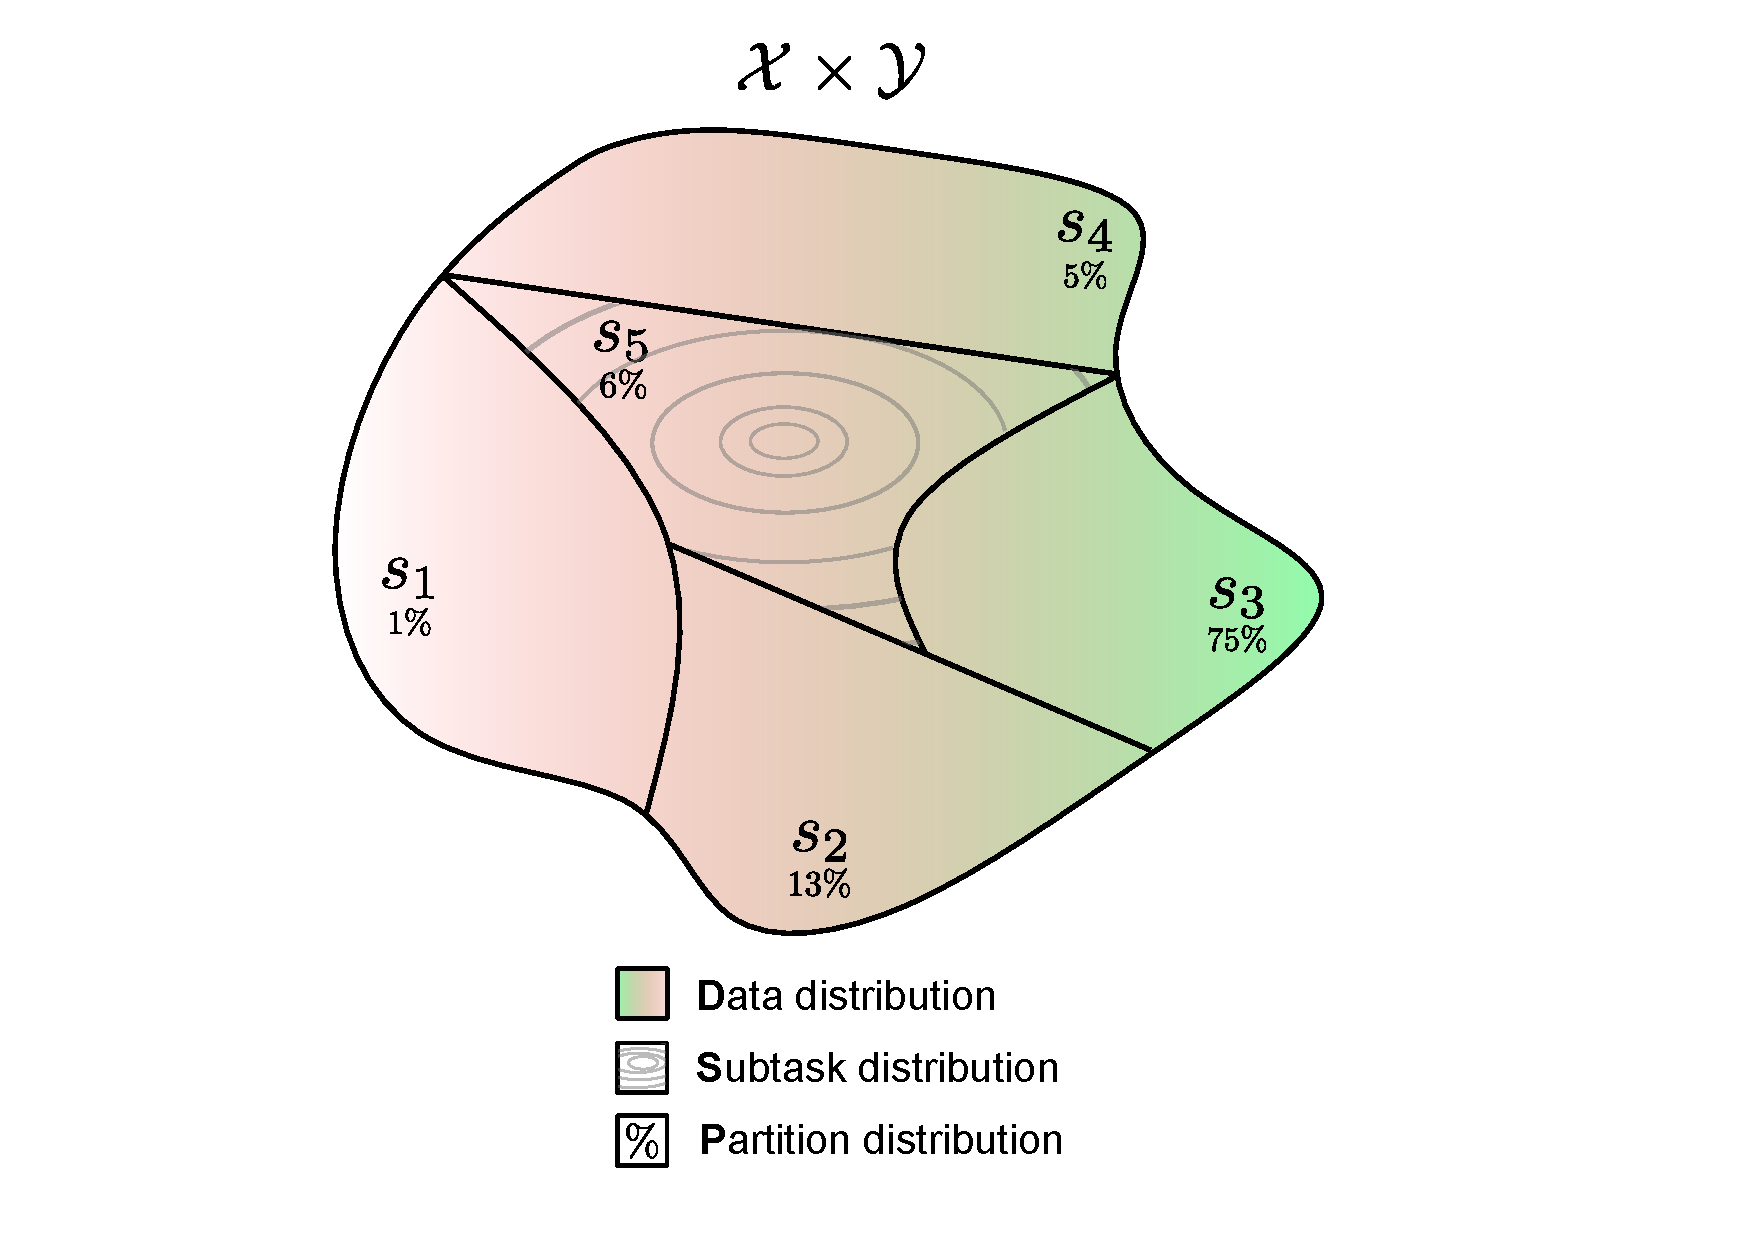
\includegraphics[width=0.5\textwidth]{figs/permissible-partition.pdf}
\caption{Starting with a data distribution $\cD$, a permissible partition
induces two additional distributions of interest: subtask distributions
(\textbf{S}), and the partition distribution (\textbf{P}). 
The underlying data
distribution of the task (\textbf{D}) is shown as a color gradient
and behaves independent of any partition. 
On the other hand, the subtask
distribution (\textbf{S}) is the data distribution conditional 
on a particular
element of the partition. Lastly, the partition distribution 
represents the probability that an input-output pair drawn from
\textbf{D} will fall in any element of the partition.}
\label{f:permissible-partition-induced-distributions}
\end{figure}
By Def.~\ref{d:permissible}, since any element of a permissible partition
has non-zero probability mass, the data distribution conditioned on this
element is well-defined and is itself also a data distribution 
(see Def~\ref{d:task}). Thus, we can now formally define the notion
of a \textit{subtask}.
\begin{defn}[Subtask]
For a given task, $T$, and its corresponding data distribution 
$\P_{\cX\times\cY}$, consider any permissible partition $\cS$ of $T$.
For any $s \in \cS$, a \textbf{subtask}, $T_s$, is the conditional
distribution
\[
\P_{\cX\times \cY | s}[A] = \P_{\cX\times \cY}[A | s]
= \frac{\P_{\cX\times\cY}[A \cap s]}{\P_{\cX \times \cY}[s]}.
\]
This last equation is the definition of conditional probability.
When it is clear from context what the permissible partition is 
we denote this distribution as $\P_s$.
\end{defn}
For any partition, we also define a discrete \textit{partition distribution}
that will come in use technically in a bit. 
\begin{defn}
For a given task $T$, parition $\cS$, the \textbf{partition distribution}
is a probability space $(\cS, 2^{\cS}, \P_\cS)$, where for all $s \in \cS$,
$\P_\cS[s] = \P_{\cX\times\cY}[s]$.
\end{defn}

% I'm not sure if taking the powerset here is ok, in particular, we need
% to make sure that this powerset sigma-algebra is a subset of the product
% sigma-algebra that was defined earlier.

\begin{rmk}
The conditions for a partition to be permissible is quite weak. Are there
perhaps more desirable conditiosn that we should require out permissble
partitions to have? Fundamentally, as the partitions get larger and larger,
it should be easier to achieve mechanistic stability. Some things to think
about:
\begin{itemize}
\item Changing ``countable collection'' to a ``finite collection''?
\item Instead of only requiring that our partitions have positive
probability mass, maybe we need that the subsets be $\eps$-representative
\citep{shalev2014understanding}.
\end{itemize}
\end{rmk}

\subsection{Causal Equivalence: A Category-Theoretic Perspective}
\label{s:causal-equiv}


\subsection{Mechanistic Stability}\label{s:mech-stab}





\section{Main results}
Herein, is a wish list of the main results that we wish to achieve.
\begin{thm}
Mechanistic stability $\Rightarrow$ in-distribution 
robustness, assuming that both $\cX, \cY$ are metric spaces. 
We also need that the task distribution $\cD_{\cX\times \cY}$ is smooth.
\end{thm}
\begin{thm}
Mechanistic stability $\Rightarrow$ in-distribution generalization.
\end{thm}
Maybe for proving this latter theorem, we can look at some proofs relating regularization.
What is a notion of in-distribution generalization that makes sense to look
at here. Can we say something stronger maybe? What about out-of-distribution?
like distribution shift?


\section{Related Literature}
What is the relationship between our notion of mechanistic stability and 
the more general notion of algorithmic stability? Is it potentially the same
as algorithmic stability applied to in-context learning?

\textbf{Algorithmic stability.} What is the relationship between algorithmic
stability and the notion of mechanistic stability that we are defining, both
in terms of the generalization bounds that are guaranteed with algorithmic
stability and in terms of the concept itself (how are we measuring
the distance between two learned hypotheses?)

\textbf{Mechanistic interpretability.} Recently, there has a been a push to interpret
neural networks by uncovering their
\textit{mechanisms}. A mechanism of a neural network with respect to some task
is a minimal subgraph of its computational graph that wholly characterizes the
network's behavior on this task~\citep{wang_interpretability_2022}. After exposing
the driving mechanisms and reverse-engineering its network into human-interpretable
components, this facilitates the understanding and improvement of models.  The general
convention has been to manually uncover the mechanisms of models. However, recent work~\citep{conmy_towards_2023}
aims to automate this process to promote work on interpretability across the field. Others 
have used concept bottlenecks~\citep{tan_interpreting_2023}, attention weight 
visualization~\citep{galassi_attention_2020}, probing feature representations~\citep{lundberg_a_2017}, and 
counterfactuals~\citep{wu_polyjuice_2021} to attempt to uncover LLMs' black-box nature. These techniques, 
though, are all domain-dependent and thus, do not allow for general interpretability of LLMs.

Our paper aims to create a generalizable metric that can be used to interpret and measure the performance 
of models across various domains and models.

\textbf{Graphical models.} Probably need to rethink the title here, we want
to explain the relationship between directed acyclic graphs, causal graphs,
and the mechanisms that we are extracting from the neural network. Our
underlying assumption is that all of these things are the same.

\section{Experimental Methods}
Can we show mechanistic stability and instability on a host of tasks?
\begin{enumerate}
\item IOI
\item Colored Objects
\item Arithmetic
\item General algorithmic tasks
\item General reasoning tasks (this and the previous task would benefit
from increased test time compute and enhanced supervision; so we can we
somehow increase stability by increasing one of these factors?)
\item General knowledge tasks (would not benefit from chain-of-thought or more
test time compute)
\end{enumerate}
What is the effect of scale on mechanistic stability? Or conversely, the benefits
that we see in terms of performance as a result of increased scale, does this
come from increased mechanistic stability?


\bibliography{references}

\newpage
\section{Category-Theoretic Causality}

\end{document}
